\documentclass[./thesis.tex]{subfiles}

 
\begin{document}

since alpha/alpha interactions are by design ignored, computation of a c\_alpha should only require knowledge of it's connection with internal space \\
SUPER costly done naively \\
list of connection supplied by QP \\
general mode \\
mircolist for connection \\
feuille de PQ to avoid duplicates \\
( custom buffers for more complex cases ) \\
repeated excitation mode(?)  \\
existing excitations are listed \\
alphas are generated through repeating excitations \\

microlisted \\
\section{def}
Idea is to create an external space and compute its influence on our selected space.
External space is only defined by c\_I\_alpha ; user should be able to only define that
By design, intern->extern and extern->extern influence isn't taken into account ( that's why it's called "external space"... )
Take into account c\_I\\alpha in the diagonalization of H : Matrix dressing
Matrix dressing
c\_I\\alpha may be derived from c ; in which case self-consistence/iteration

\section{task splitting}

Load balancing is a major issue in parallel computing. Often, the tasks we intuitively would like to create have very different computing times. In several of our algorithms, we faced the problem of a few tasks being considerably longer than the others. We took a generic approach of defining a ``fragmentation'' level $F_i$ for all ``logical'' tasks $i$, defining a number of independent ``actual'' tasks it should be decomposed in, based on its estimated cost. Task $i$ is put in the job queue $F_i$ times, each time associated with and index $s$ ranging from $0$ to $F_i-1$.

In practice, $F_i \neq 1$ is only found for the few very expensive tasks.
There is of course no universal approach to define a task sub-division, but a generic way is to set a counter $c$ at the begining of a loop and skip it if $s \neq c \mod F_i$.

Imagining a toy problem where we have $M$ a list of $N$ matrices size $n \times n$, and for each $M^i$ we want to print

\begin{equation}
\sum_{x} \sum_y \text{transmogrify}(M^i_{xy})
\end{equation}

with $\text{transmogrify}$ some expensive computation, the pseudo-code for the master and slave could be as shown in algorithm \ref{alg:tasksplit_master} and \ref{alg:tasksplit_slave} respectively.


\begin{algorithm}
	\label{alg:tasksplit_master}
	\caption{tasksplit\_master}
	\tcc{A logical task is computation for one matrix}
	chose $F_i$ \;
	\For{$i=1,N$}{
	\For{$s=0,F_i-1$}{
		add task $(i,s)$ to the queue	
	}
	}
	$f$,$\text{R}$ are arrays size $N$ initialized with $0$ \;
	\While{not all matrices printed}{
		get $(i,\text{sum})$ from a slave \;
		$R[i] \gets R[i] + \text{sum}$ \;
		$f[i] \gets f[i] + 1$ \;
		\If{$f[i] = F_i$}{
			print $R[i]$ \;
		}
	}
\end{algorithm}

\begin{algorithm}
	\label{alg:tasksplit_slave}
	\caption{tasksplit\_slave}
	\While{}{
		get task $(i, s)$ from the queue \;
		$R \gets 0$ \;
		$c \gets 0$ \;
		\For{$x=1,n$}{
		\For{$y=1,n$}{
			$c \gets c + 1$ \;
			\If{$s = c \mod F_i$}{
				$R \gets R + \text{transmogrify}(M^i_{xy})$ \;
			}
		}
		}
		send result $(i, R)$ \;
	}
\end{algorithm}

\section{implementation}
Plein de variable, subsection pour resumer la notation?
For clarity, indices will be named depending on what they refer to
\begin{itemize}
\item
$i,j$ refer to samples/generator determinants
\item
$m$ refers to checkpoints
\item
$t$ refers to teeth
\end{itemize}

In some respect, computing the dressing vector is akin to computing PT2. Matrix dressing can be seen as a sum of elementary dressing vectors $\delta(\alpha)$, each one associated with a particular $\ket \alpha$, just like PT2 is a sum of $\epsilon(\alpha)$. It is possible to pack those elementary vectors together like we packed $\ket \alpha$ together for PT2.

\begin{equation}
\Delta_I = \sum_{\alpha \in \mathcal{A}_I} \delta(\alpha)
\end{equation}


\begin{equation}
\Delta = \sum_{I} \Delta_I
\end{equation}

Thus, both are a sum over all external determinants, and require to find connections between those determinants and the internal wavefunction. Presumably, the norm of resulting elementary dressing vectors $\Delta_I$, will scale in a fashion similar to that of $e_I$.
With that in mind, is seems possible, theoritically, to generalize our hybrid stochastic-deterministic PT2 for computing dressing vectors.
However there are a few significant difference.
\begin{itemize}
\item
We were estimating a scalar, now we are estimating a vector. What should the error bar refer to?
\item
In both cases we have $N_{gen}$ samples, however for PT2 each sample is a scalar, here each sample is a vector size $N_{det}$. It is easy to store $N_{gen}$ scalars, not to store $N_{gen}$ vectors size $N_{det}$
\item
In the case of PT2 ( at least in it Epstein-Nesbet version ), each connection found, only requires an increment of some elements of $P(G_{pq})$. At no point 2 connections need to be known at the same time. This is different for methods implemented with matrix dressing( or even with other version of PT2? ). It is possible that the detail of which variational determinants a $\ket \alpha$ connects to, needs to be known in ordrer to be able to compute $delta_\alpha$.
\end{itemize}

To address the first problem, we decided to compute the error bar for $E_{\Delta}$ the energy contribution of $\Delta$. Our dressed matrix being $H + \Delta$, its energy is
    
\begin{equation}
\frac{\langle \Psi |H + \Delta | \Psi\rangle}{\langle \Psi | \Psi \rangle} = \frac{\langle \Psi |H  | \Psi\rangle}{\langle \Psi | \Psi \rangle} + \frac{\langle \Psi |\Delta | \Psi\rangle}{\langle \Psi | \Psi \rangle} = E_H + E_{\Delta} 
\end{equation}


$E_{\Delta}$ will be estimated the same way as $E_{PT2}$ was, based on idividual contributions $e_{\Delta_I}$

\subsection{storage}

The core idea is that, in a Monte-Carlo scheme, even an "exotic" one like our own, the estimated result has to be a linear combination of all samples. At any point $m$ of the Monte-Carlo computation corresponding to $M_m$ combs having been drawn, we can write our estimated dressing vector $\Delta^m$ as :


\begin{equation}
\Delta^m = \sum_{I=1}^{N_{gen}} \epsilon^m_{I} \Delta_I
\end{equation}


The values for $\epsilon^m_I$ have no dependence on those of $\Delta_I$. They only depend on what samples have been drawn so far. Since we decide beforhand which combs are going to be drawn, we can compute $\epsilon$ vector for any point of the Monte-Carlo before any sample has been computed. The values we chose for $M_m$ act as predetermined "checkpoints".

%This allows us to set up "checkpoints" for predetermined values of $n$. These value are refered to as $M_m$ with $M_0 = 0$ and $M_m < M_{m+1}$.

\begin{figure}[h!]
	\begin{center}
		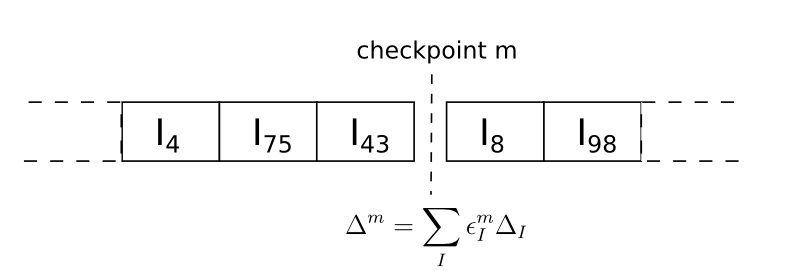
\includegraphics[width=1.00\columnwidth]{figures/matrix_dressing/checkpoint}
		\caption{\label{checkpoint}}
		CONFUSION ENTRE CHECKPOINT ET DENT POSSIBLE, RENDRE VERTICAL?
	\end{center}
\end{figure}



Those checkpoints can be set at any arbitrary point, but they must be determined beforehand and cannot be changed during the computation ; we will only be able to get results at those points.
For checkpoint $m$, we start with a null vector $\tilde \Delta^m$. Each time an elementary vector $\Delta_I$ is computed
we increment it 



\begin{equation}
\tilde \Delta^m \gets \tilde \Delta^m + \epsilon_I^{m} \Delta_I
\end{equation}


Once this has been done, $\Delta_I$ can be discarded. Indeed, when checkpoint $m$ is reached, $\tilde \Delta^m = \Delta^{m}$, as obviously $\epsilon_I^{m} = 0$ for any $\Delta_I$ sample that hasn't yet been drawn at checkpoint ${m}$.
For convenience, some notations we defined can be adapted as functions of a checkpoint reached

\begin{equation}
\dot t_m = t_{M_m}
\end{equation}
the first non-deterministic tooth when checkpoint $m$ is reached, and

\begin{equation}
\dot n_0(m) = n_0(t_{M_m})
\end{equation}

the size of the deterministic range when $m$ is reached.


$\epsilon$ is defined as follow

\begin{equation}
\epsilon^m_i = 
\begin{cases}
1 & \text{if } i \leq \dot n_0(m) \\
\frac{W_T \times M_{m,i}}{w_i \times M_m} & \text{if } i > \dot n_0(m)
\end{cases}
\end{equation}


with $M_{m,i}$ the number of times sample $i$ has been drawn at checkpoint $m$.


The memory cost for a checkpoint $m$ is $2 \times N_{det}$ floats, corresponding to the storage of $\epsilon^m$ and $\tilde \Delta^m$. This cost is small enough to allow setting up quite a few checkpoints. However, in addition to this memory cost, comes some computational cost. If we set up $N_{cp}$ checkpoints, it implies each time a sample is drawn, we will have, theoretically, to incremement $N_{cp}$ vectors of size $N_{det}$. For quicker jobs, this price may not be negligible. It gets worse if, as was the case in our first implementations, a collector is in charge of updating checkpoints for multiple slaves. 


We can drastically reduce the amount of writting required for each sample by rewriting $\Delta^m$.
Firstly, we define $\Delta^{D,t}$ as the total dressing for teeth $t$
\begin{equation}
\Delta^{D,t} = \sum_{I \in P_t} \Delta_I
\end{equation}

We rewrite $\Delta^m$ as

\begin{equation}
\label{eq:rewrite1}
\Delta^{m} = \sum_{t=0}^{\dot t_m - 1} \Delta^{D,t}+ \sum_{I=1}^{N_{gen}} \gamma^m_{I} \Delta_I
\end{equation}

The second term being $\Delta^m$ minus its deterministic contribution, we can trivially write

\begin{equation}
\gamma^m_i = 
\begin{cases}
0 & \text{if } i \leq \dot n_0(m) \\
\epsilon^m_i = \frac{W_T \times M_{m,i}}{w_i \times M_m} & \text{if } i > \dot n_0(m)
\end{cases}
\end{equation}

We define

\begin{align}
\Delta^{S,m} = \sum_I (\gamma^m_I - \gamma^{m-1}_I) \Delta_I \\
\end{align}

We can rewrite the second term of equation \ref{eq:rewrite1}
\begin{equation}
\sum_{I=1}^{N_{gen}} \gamma^m_{I} \Delta_I = \sum_{p<m} \Delta^{S,p}
\end{equation}

And write the final form or $\Delta^m$ as
\begin{equation}
\Delta^m=\sum_{t=0}^{\dot t_{m}-1} \Delta^{D,t} + \sum_{p \leq m} \Delta^{S,p}
\end{equation}

The vectors we need to store are $\Delta^{D,t}$ and $\Delta^{S,m}$. Each time we compute an elementary dressing vector $\Delta_I$, the need for update goes as follow

\begin{itemize}
\item
$\Delta^{D,t}$ with $I \in P_t$. This is exactly one write.
\item
$\Delta^{S,m}$ where $\gamma^m_I - \gamma^{m-1}_I \neq 0$. This is
 \begin{itemize}
 \item
 	No write if it is moved to the deterministic set in the same checkpoint it is first drawn or computed for tooth filling
 \item
 	Otherwise, one write per checkpoint in which it is drawn until the one where it is moved to the detemrinistic set, inclusive.
 \end{itemize}
 While this retains the maximum of $N_{cp}$ writes for one sample, it is much lower in practice.
\end{itemize}

For convenience we define

\begin{equation}
\tilde \epsilon^m_I = \gamma^m_I - \gamma^{m-1}_I
\end{equation}

\begin{comment}
We can drastically reduce the amount of writting required for each sample, by separating the deterministic and stochastic part, and computing differences between checkpoints rather than checkpoints directly.
For the deterministic part, things are straightforward. We allocate a vector $\Delta^{D,t}$ of size $N_{det}$ for each tooth $t$, and one $\Delta^{D,0}$ for the initial deterministic set. For each sample that is computed, the $\Delta^{D,t}$ vector corresponding to the $t$ tooth it belongs in - or $\Delta^{D,0}$ if it belongs in the initial deterministic part - is incremented. That's exactly 1 vector write per sample.




For the stochastic part, instead of using $\epsilon$, we use $\tilde \epsilon$, defined as follow.

\begin{equation}
\tilde \epsilon^m_i = 
\begin{cases}
0 & i \leq \dot n_0(m) \\
\frac{W_T \times (M_{m,i}-M_{m-1,i})}{w_i}  & i>\dot n_0(m)
\end{cases}
\end{equation}




\begin{equation}
\tilde \epsilon^m_i = 0 ; i \leq rDetI[m]
\end{equation}



\begin{equation}
\tilde \epsilon^1_i = acw[1] \times n[1,i]  ; i>rDetI[1] ??
\end{equation}



\begin{equation}
\tilde \epsilon^m_i = acw[i] \times (n[m,i]-n[m-1,i])  ; i>rDetI[m]; m>1 ??
\end{equation}


(notation  $\tilde \Delta^m$ utilise aussi pour $\epsilon$ )
As can be seen, $\tilde \Delta^m$ will need to be updated when sample $i$ is computed, only if $M_{m,i}-M_{m-1,i} \neq 0$, in other word, only if $i$ has been drawn between checkpoint $m-1$ and $m$. [This means at most 1 writting ( instead of $N_{cp}$ ) each time a sample is drawn.]FAUX? 

$\epsilon$ can be reconstructed from $\tilde \epsilon$.




\begin{equation}
\epsilon^m_i =
\begin{cases}
1 & i \leq \dot n_0(m) \\
\frac{1}{M_m} \sum_{p=1}^{m} {\tilde \epsilon^p_i} & i > \dot n_0(m)
\end{cases}
\end{equation}



$\epsilon^m_i$ is not explicitely reconstructed in the shown algorithms, $\Delta^m$ is directly computed from $\tilde \epsilon^m_i$.
\alert{A VERIFIERXXXXXXXXXXXXXXXXXXXXXXX}
\begin{equation}
\Delta^m=\Delta^{D,0} + \sum_{t=1}^{\dot t_{m}-1} \Delta^{D,t} + \sum_{p \leq m} \tilde \Delta^p
\end{equation}
\end{comment}


\begin{algorithm}
	\caption{OPTIMIZE\_MONTECARLO}
	\label{OPTIMIZE_MONTECARLO}
	
	%\SetKwFunction{FMain}{OPTIMIZE\_MONTECARLO}
	%\SetKwProg{Fn}{Function}{:}{}
	
	%\Fn(\tcc*[h]{Optional algorithm to reorder jobs so checkpoints are reached as fast as possible.}){\FMain{some args}}{
		$R^{-1}$ so that $R^{-1}[R[i] > 0] = i$ \;
		\tcc{checkpoint $m$ is reached when the first $R^{-1}[m]$ jobs are done}
		$lastNj \gets 1$ \;
		\For{$m=1,N_{cp}$}{
			$Nmoved \gets 0$ \;
			\For{$j=lastNj,R^{-1}[m]$}{
				\If{$M_{m,J_j} = 0 \& J_j > \dot n_0(m)$}{
					\tcc{ensures moved jobs are at the end of the checkpoint once sorted}
					$J_j \gets J_j + N_{gen}$ \;
					$Nmoved \gets Nmoved + 1$ \;
				}
			}
			sort array J from $lastNj$ to $R^{-1}[m]$, inclusive \;
			\tcc{moved jobs are sent to the next checkpoint}
			$R^{-1}[m] \gets R^{-1}[m] - Nmoved$ \;
			\tcc{restores moved jobs original value}
			\For{$j=R^{-1}[m]+1,R^{-1}[m] + Nmoved$}{
				$J_j \gets J_j - N_{gen}$ \;	
			}
			$lastNj \gets R^{-1}[m] + 1$ \;
		}
		$R[*] \gets 0$ \;
		%$R[R^{-1}[1]] = 1$ \;
		$\tilde R \gets 0$ \;
		$k \gets 0$ \;		
		\For{$i=1,N_{cp}$}{
			\If{$R^{-1}[i] \neq \tilde R$}{
				$k \gets k + 1$ \;
				$\tilde R \gets R^{-1}[i]$ \;				
				$R[\tilde R] = k$ \;
			}
		}
		$N_{cp} \gets k$ \;
\end{algorithm}

Algorithm (Nmoved) is an optional reorganization of jobs order. It doesn't change the result for any checkpoint, but only ensures it is available as quickly as possible. It takes two things into consideration:
\begin{itemize}
\item
Because no result is available between two checkpoints, the order in which jobs are processed between two checkpoints is irrelevant for the result. So, as is usually the case with parallel jobs, we would like to do the longest tasks first, so that we don't get an extra delay due to a massive task being done last. Therefore, jobs should always be in ascending order ( descending computational time N'A PAS ETE EXPLIQUÉ) between two checkpoints.
\item
Because of the "tooth filling", sometimes samples computed inside a checkpoint aren't useful for the result. Since tooth filling picks the first uncomputed jobs, they are of high computational cost. The algorithm iterates over checkpoints in ascending order, each time moving such sample to the next checkpoint. Thus, every sample is moved to the first checkpoint it's actually involved in, either deterministically or stochastically.
\end{itemize}



\begin{algorithm}
	\caption{PRECOMPUTE\_MONTECARLO}
	\label{PRECOMPUTE_MONTECARLO}
	\tcc*[h]{Computes $J$ the array so that $J_i$ is the $i^{th}$ sample that must be computed to perform the Monte-Carlo computation, and $n[m,i]$ the total number of times sample $i$ has been drawn at checkpoint $m$, regardless of which teeth are in the deterministic part.}
	
		$\tilde M$ array size $\Ndet$ initialized with $0$\;		
		$N_c \gets 0$ \;
		$N_j \gets n_0(1)$ \;
		\For{$i=1,N_j$}{
			$d_i \gets TRUE$ \;
			$J_i \gets i$ \;
		}
		
		$m \gets 1$ \;
		$F \gets N_j+1$ \;
		\While{$N_j < N_{gen}$}{
			ADD\_COMB shown as algorithm \ref{alg:FILL_TOOTH} \;
			FILL\_TOOTH shown as algorithm \ref{alg:ADD_COMB} \;
		  
		  
		  %$oldcurth \gets curth$ \;
		  %\While{$curth \leq N_{cpmax}$}{
		  %	\If{$N_j \leq cpthreshold[curth]$}{
		  %		$curth \gets curth + 1$ \;
		  %	}
		  %}
		  
		  \If{$M_m = N_c$}{
		  	$R[N_j] \gets m$ \;
		    %$cpthreshold[m] \gets N_j$ \;
            $M_{m,*} \gets \tilde M$ \;
            $m \gets m+1$ \;
		  } 
		}
\end{algorithm}



\begin{algorithm}
	\label{COMPUTE_EPSILON}
	\caption{COMPUTE\_EPSILON}
		\KwResult{ $\tilde \epsilon$}
		$\epsilon^*_* \gets 1$ \;
		$F \gets 1$ \;		
		\For{$m=1,N_{cp}$}{
			\While{$F \leq N_{gen}$}{
				\uIf{$M_{m,F} \neq 0$}{
					$F \gets F+1$ \;
				}\Else{
					break \;
				}
		  	}
		  	$\dot t_m \gets N_{teeth}+1$ \;
			$\dot n_0(m) \gets N_{gen}$ \;
			\For{$t=2,N_{teeth}+1$}{
				\If{$F-1 \leq n_0(t)$}{% rTeethI[t]$}{
					$\dot t_m \gets t-1$ \;
					$\dot n_0(m) \gets n_0(t-1)$ \;
					break loop \;
				}
			}
			
			
			\For{$t=\dot t_m,N_{teeth}$}{
				
				\For{$i=n_0(t)+1,n_0(t+1)$}{
					$\tilde \epsilon^m_i \gets \frac{W_T \times M_{m,i}}{w[i]}$ \;
				}
			}
		}
		\For{$m=N_{cp},2,step=-1$}{
			$\tilde \epsilon^m_* \gets \tilde \epsilon^m_* - \tilde \epsilon^{m-1}_*$ \;
		}
\end{algorithm}

\begin{algorithm}
	\tcc{code for a slave node, OMP parallel}
	
	cp\_done, cp\_sent : shared scalars initialized to $0$ \;
	cp\_max : shared array size $N_{proc}$ initialized to $0$ \;
	
	
	\tcc{loop for each core $iproc$}
	\While{}{
		try to get task $(I,s)$ from queue \;
		\uIf{task was available}{
			\alert{pas de notaion pour l'ensemble d'un checkpoint} \;
			$m$ so that $I \in CHECKPOINT_m$ \;	
		}\Else{
			$m \gets N_{cp} + 1$ \;		
		}
		will\_send $\gets 0$ \;
		--OMP CRITICAL-- \;
		cp\_max$[iproc] \gets m$ \;
		cp\_done $\gets min(\text{cp\_max}) -1$ \;
		\If{cp\_done > cp\_sent}{
			will\_send $\gets$ cp\_done \;		
			cp\_sent $\gets$ cp\_done \;		
		}
		--END OMP CRITICAL-- \;
		\If{will\_send $\neq 0$}{
			SEND $\Delta^{\text{will\_send}}$ shown in algo TBD
		}
		\If{$m = N_{cp}+1$}{
			exit \;
		}
		UPDATE with I shown in algo TBD \;
	}
\end{algorithm}

\begin{algorithm}
	\tcc{UPDATE}
	\KwData{global shared scope : $\Delta^{D,t}$ and $\tilde \Delta^{m}$ as described, initialized with $0$}
	\KwData{global shared scope : $f$ an array size $N_{gen}$ initialized with $0$. The fragmentation count}
	
	\KwData{from outer scope : $s, I \in CHECKPOINT_m$} 
	\BlankLine
	$t$ so that $I \in P_t$ \;
	\alert{notation pour fragmentation pas defini}
	
	compute $\Delta_{I,s}$ ($\Delta_{I}$ avec fragmentation index $s$ ...) \;
	\tcc{lock global arrays before update}
	$\Delta^{D,t} \gets \Delta^{D,t} + \Delta_I$ \;
	\For{$m'=m,N_{cp}$}{
		\If{$\tilde e^m_I \neq 0$}{
			$\tilde \Delta^{m'} \gets \tilde \Delta^{m'} + \frac{W_T}{w_I} \Delta_I$ \;
		}
	}
	$e_{\Delta_I} \gets e_{\Delta_I} + C \cdot \Delta_{I,s}$ \;
	$f[I] \gets f[I] + 1$ \;
\end{algorithm}


\begin{algorithm}
	\tcc{SEND}
	
	\tcc{compute partial value of $\Delta^m$ with partial values of $\Delta^{D,t}$ and $\tilde \Delta^m$}
	
	$\Delta^m \gets 0$ \;
		\For{$m'=m,1$}{
				\alert{erreur sur le facteur?} \;
				$\Delta^m \gets \Delta^m + \frac{\tilde \Delta^{m'}}{M_m}$
			}
			
			\For{$t=t-1,0,-1$}{
				$\Delta^m \gets \Delta^m + \Delta^{D,t}$ \;
			}
			
			
			
	$\mathcal{I}$ the set of $I \in CHECKPOINT_m$ with $f[I] > 0$ \;
	send ($\Delta^m$, $\mathcal{I}$, $e_{\Delta_{I \in \mathcal{I}}}$, $f[I \in \mathcal{I}]$)
\end{algorithm}

\begin{algorithm}
	get ($\breve \Delta^m$, $\mathcal{I}$, $\breve e_{\Delta_{I \in \mathcal{I}}}$, $\breve f[I \in \mathcal{I}]$) \;
	$\Delta^m \gets \Delta^m + \breve \Delta^m$ \;
	\ForAll{$I \in \mathcal{I}$}{
		$\breve e_{\Delta_{I}} \gets \breve e_{\Delta_{I}} + \breve e_{\Delta_{I}}$ \;
		$f[I] \gets f[I] + \breve f[I]$ \;
	}
	
	treat $e_{\Delta_{I}}$ as $e_I$ in the pt2 algorithm to estimate error \;
\end{algorithm}

\subsection{finding connections - microlists}

For merely enumerating the connections between internal and external space, there are two possible ways.
Internal to external, or External to internal
%\begin{figure}[h!]
	\begin{center}
		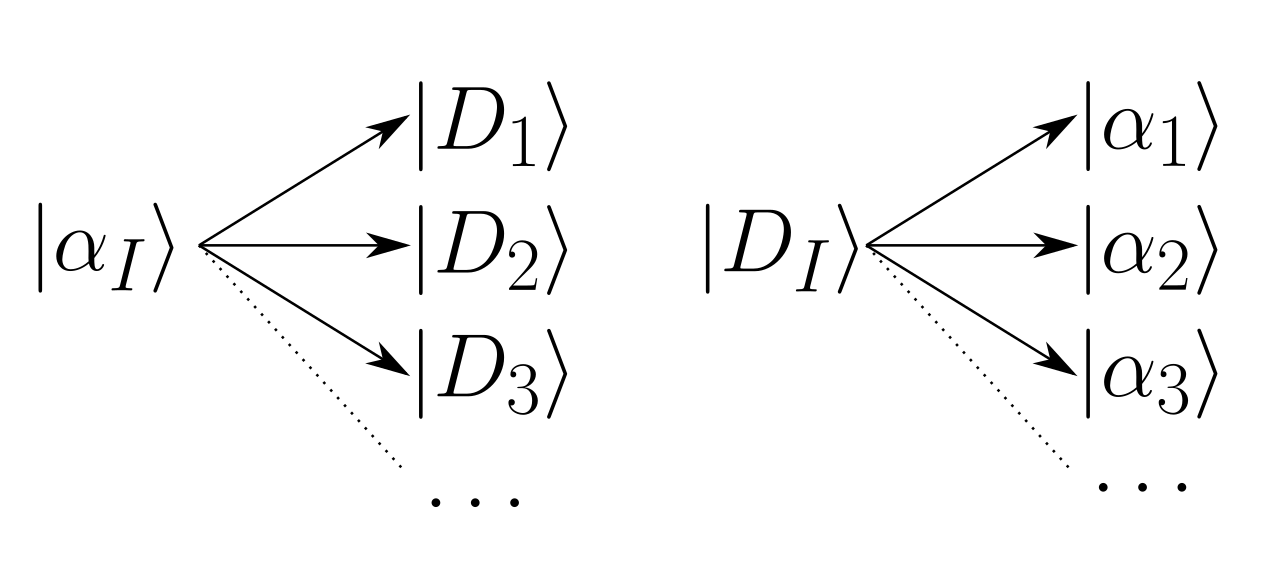
\includegraphics[width=0.5\columnwidth]{figures/matrix_dressing/interactions}
		%\caption{\label{interactions}}
	\end{center}
%\end{figure}

Computation-wise, those two possbilities are very different.

The internal to external approach is pretty straightforward, as it means applying every possible double excitation to all determinants of an arbitrary set $\Psi$ of size $N_{det}$. The only difficulty is to ensure the created $\alpha$ are actually external to $\Psi$. We did this and more in our CIPSI implementation.

The external to internal approach is more difficult as it means finding connections between all determinant $\alpha$ in an arbitrary set size $N_{external}$ - typically a few orders of magnitude larger than $N_{det}$ - and a set of abritrary determinants $\Psi$. 

Unfortunately, we typically need to know all connection for a particular $\alpha$ before we can compute its associated dressing vector, which puts us in the internal to external case.

In our CIPSI algorithm, we are only considering $N_{virt}^2$ $\alpha$ at the same time. We can build, for each of those $\alpha$, a list of connected $I$ that we incrementally build from connections we find by internal-to-external approach.


However, the storage space for the worst-case scenario isn't sustainable. ( a reformuler/clarifier ptet)
$G_{pq}$ being the first batch, and the variational wavefuction being all determinants up to quadruply excited from $G$ except those in the $G_{pq}$ batch. There are $~ N_{virt}^2$ unique $\alpha$ in the batch. For each of them, any of the $~N_{occ}^2 N_{virt}^2$ double excitation will lead to a variational determinant, except if it leads to one of the $N_{virt}^2$ determinant of the batch.
We have $~ N_{virt}^2$ alpha each connected to $~(N_{occ}^2-1) N_{virt}^2$ variational determiants, resulting in a storage space $~N_{occ}^2 N_{virt}^4$.
Even in the more realistic case where half of double excitations involving the holes in the HOMO of the HF determinants are present in the internal space, storage needed for the ionzied generator $a_{\bar{HOMO}} a_{HOMO} HF$ will be $N_{virt}^4 / 4$, which, depending on the system size, may be concerningly or prohibitively high. 

(PREUVE?)

\begin{algorithm}
	\label{BUILD_CONNECTED}
	\caption{BUILD\_CONNECTED}
		\KwData{ ---------}
		\KwResult{ ------------}
        $i_1 = N$ \;   
        $L_{1..i_1} \gets D_{1..{i_1}}$ \;
		\ForAll{$r ; B_{r0}$}{
		\tcc {$B_{r0} = FALSE$ if column entirely tagged}
		  $i_2 = i_1 + N^r$ \;
		  $L_{i_1+1..i_2} \gets D^r_{1..N^r}$ \;
		  \For{$i=1,N_r$}{
		    $T_{D^r_i} \gets FALSE$
		  }
		  \ForAll{$s ; B_{s0}$}{
		    $i_3 = i_2$ \;
		    \For{$i=1,N_s$}{
		      \If{$T_{D^s_i}$}{
		        $i_3 \gets i_3+1$ \;
		        $L_{i_3} \gets D^s_i$ \;
		      }
		    }
		    
		    $i_4 = i_3 + N^{rs}$ \;
		    $L_{i_3+1 .. i_4} \gets D^{rs}_{1..N^{rs}}$ \;
		    \tcc{$L$ is the list of all $I \in \Psi ; EXC(I, a^\dagger_r a^\dagger_r G_{pq} ) \leq 2$}
		  }
		 \For{$i=1,N_s$}{
		    $T_{D^r_i} \gets TRUE$
		  }
		}
\end{algorithm}



\begin{algorithm}
	\label{BUILD_MICROLIST}
	\caption{BUILD\_MICROLIST}
		\KwData{ ------}
		\KwResult{ ------}
        $N \gets 0$ \;
        $N^* \gets 0$ \;   
        $N^{*,*} \gets 0$ \;    
        \ForAll{$I \in \{S - past\} ; f_{G_{pq}}^I \leq 4$}{
          $(P,H) \gets particles\_and\_holes(G_{pq}, I)$ \;
          $p = list\_from\_bitstring(P)$ \;
          
          %$h = LIST_FROM_BITSTRING(H)$
          \uIf{$f_{G_{pq}}^I = 4$ \& $B_{p_1,p_2}$}{
            $i \gets N^{p_1, p_2}+1$ \;
            $N^{p_1, p_2} \gets i$ \;
            $D^{p_1, p_2}_{i} \gets I$ \;
          }
          \uElseIf{$f_{G_{pq}}^I = 3$ \& $B_{p_1}$}{
            $i \gets N^{p_1}+1$ \;
            $N^{p_1} \gets i$ \;
            $D^{p_1}_{i} \gets I$ \;
          }
          \Else{
            $i \gets N+1$ \;
            $N \gets i$ \;
            $D_{i} \gets I$ \;
          }
        }
\end{algorithm}




\section{Alpha-factory (rename?)}


General framework which allows to create methods with minimal effort 

\section{parallel}
just like pt2 stoch, 1 task = 1 generator \\
however, 1 result = 1 vector instead of 1 scalar \\
additional difficulties \\
memory: \\
to avoid N\_det\^2, checkpoints \\
communication \\
4 scalars per checkpoint \\



\end{document}
